\section{Calibrated pair energies}\label{sec:18.4}

Back at keV deposits, where two moments describe the pair number, a charge-resolving silicon sensor at \SI{123}{K} measures $\varepsilon_{\mathrm{eh}} = \SI{3.749 \pm 0.001}{eV}$ and $F_{\mathrm{eh}} = 0.119 \pm 0.002$ for \SI{5.9}{keV} X-rays~\cite{rodrigues2021absolute}. The cascade of \cref{sec:18.1,sec:18.2}, reduced to energy alone and given free-particle kernels, has one constant that a measurement must fix. Once the measured $\varepsilon_{\mathrm{eh}}$ fixes the constant, the cascade predicts $F_{\mathrm{eh}}$. It predicts both numbers for every other crystal as well, including the crystals ranked in \cref{chap:17}, for most of which neither number has been measured. A guide to new targets needs a pair energy for each crystal, and it needs to know which of these pair energies rest on comparison with data. With its one constant fixed in silicon, the cascade comes within 5 to \SI{6}{\percent} of the measured pair energies of germanium and GaAs, and its pair energies reduce to the line $\varepsilon_{\mathrm{eh}} \approx 1.61\Eg + k_2$.

\subsection{The calibrated cascade}\label{sec:18.4-model}

The model is the random-$k$ cascade of \cref{sec:18.1-reductions} with free-particle densities of states, threshold ratio $\theta_{\mathrm{ii}} = 1$, one optical phonon of energy $\omega_{\mathrm{AB}}$ and, in silicon, a hole band cut at $B_{\mathrm{h}} = \SI{12}{eV}$, solved by the moment recursions of \cref{sec:18.2-heat}. In units of the gap the model depends on a crystal through the two numbers defined in \cref{sec:18.2-heat}, the phonon strength $\lambda_{\mathrm{AB}} = A_{\mathrm{AB}}/\Eg^3$ and the phonon step $w_{\mathrm{AB}} = \omega_{\mathrm{AB}}/\Eg$. A cascade with large $\lambda_{\mathrm{AB}}$ loses most of its energy to phonons on the way down and settles more slowly: germanium, with $\lambda_{\mathrm{AB}} > 5$, needs slopes fitted for seed energies between 30 and $60\Eg$, against 20 to $40\Eg$ for silicon. All values are the continuum limit of the recursions.

The constant is fixed in silicon. With $\Eg = \SI{1.160}{eV}$ at \SI{123}{K}~\cite[Eq.~(11)]{ramanathan2020ionization} and $\omega_{\mathrm{AB}} = \SI{63}{meV}$, the measured pair energy requires
\begin{equation}
  A_{\mathrm{AB}} = \SI{5.703}{eV^3} ,
  \label{eq:18.4-AAB}
\end{equation}
so that $\lambda_{\mathrm{AB}} = 3.65$ and $w_{\mathrm{AB}} = 0.0543$ for silicon. The same constant leads to $F_{\mathrm{eh}} = 0.114$ (\cref{sec:18.2-silicon}). This value of $A_{\mathrm{AB}}$ lies \SI{10}{\percent} above the 5.2 that Alig and coworkers fitted to the pair energy of silicon~\cite[Sect.~II]{nielsen2026first}. With 5.2 and the room-temperature gap of \SI{1.12}{eV}, the same cascade gives \SI{3.64}{eV}, inside the range of 3.62 to \SI{3.66}{eV} measured at \SI{300}{K}~\cite[Table~I]{ramanathan2020ionization}. Everything else in this section uses \cref{eq:18.4-AAB} unchanged: one constant for all crystals. The universality of the constant is an assumption, and the comparison with other crystals tests it.

Two cascade calculations with no constant left to fit exist for silicon. Nielsen and Fischetti use density-functional bands and phonons, a loss-function kernel without exchange and a plasmon channel, and find $\varepsilon_{\mathrm{eh}} = \SI{3.10}{eV}$ with a time-dependent density-functional loss function and \SI{3.50}{eV} with a $GW$/Bethe--Salpeter one~\cite[Sect.~III]{nielsen2026first}; they apply the same method to six of the crystals below (the last column of \cref{tab:18-valid}). The full-band cascade of \cref{sec:18.3-fullband} uses empirical pseudopotential bands and deformation-potential phonons and gives $\varepsilon_{\mathrm{eh}} = \SI{4.15}{eV}$, with the envelope $[3.95, 4.73]$~eV of its variants. The class of model adds a systematic of at least $\pm\SI{0.4}{eV}$, taken from the shift between the two loss functions of Nielsen and Fischetti. Without a fitted constant, Nielsen and Fischetti lie below the measured \SI{3.749}{eV} and the full-band cascade above it. The two calculations do not meet even with matched ingredients: with first-principles phonon couplings for both carriers and without exchange, as Nielsen and Fischetti have them, the full-band cascade still gives \SI{4.11}{eV}, and the remaining difference of \SI{0.6}{eV} from their \SI{3.50}{eV} is unexplained. The unexplained difference lies where the pair energy is decided, in the rate of impact ionization between threshold and about \SI{4.5}{eV} (\cref{sec:18.1-reductions}). At \SI{100}{eV} the full-band cascade turns \SI{71.6}{\percent} of the deposit into heat, with the envelope $[70.2, 75.0]$~\si{\percent}.

\subsection{Silicon, germanium and GaAs}\label{sec:18.4-three}

\Cref{tab:18-pairs} sets the model against the measurements. Each crystal is computed twice: at the gap of the measurement temperature, for the comparison, and at its low-temperature gap of \cref{tab:3-materials}, for a detector at millikelvin. Temperature enters the model only through $\Eg(T)$. Leaving out phonon absorption costs little: the occupation of the \SI{37.6}{meV} germanium phonon is 0.0035 at \SI{77}{K}. The phonon energy $\omega_{\mathrm{AB}}$ is the measured zone-center optical energy, \SI{37.6}{meV} for germanium (\cref{tab:5-phonons}) and the longitudinal \SI{36.35}{meV} for GaAs (\cref{sec:5.5}); neither crystal has a hole cutoff.

\begin{table}[tbp]
\caption{Mean energy per pair and Fano factor of the energy-only random-$k$ cascade with the single constant \cref{eq:18.4-AAB}, against measurements. Germanium gap at \SI{77}{K} from the fit of Wei, Wang and Mei~\cite[Eq.~(7)]{wei2016average}; other gaps from \cref{tab:3-materials} and \cref{app:E.13}. Measurements: silicon~\cite{rodrigues2021absolute}; germanium, the pair energy and the range of five Fano-factor experiments quoted by Mei and coworkers~\cite[Sect.~4.3]{mei2020impact}; GaAs, the room-temperature value of Bertuccio and Maiocchi as quoted by Nielsen and Fischetti~\cite[Fig.~1]{nielsen2026first}. Residual: model over measured, minus one.}
\label{tab:18-pairs}
\centering\small\setlength{\tabcolsep}{4pt}
\begin{tabular}{llccccc>{\raggedright\arraybackslash}p{0.2\linewidth}}
\toprule
 & $T$ & $\Eg$ (eV) & \multicolumn{2}{c}{$\varepsilon_{\mathrm{eh}}$ (eV)} & \multicolumn{2}{c}{$F_{\mathrm{eh}}$} & Status \\
 & & & model & measured & model & measured & \\
\midrule
Si & \SI{123}{K} & 1.160 & 3.749 & $3.749 \pm 0.001$ & 0.114 & $0.119 \pm 0.002$ & $\varepsilon$ fitted; $F$ predicted, $2.4\sigma$ low \\
 & low & 1.17 & 3.766 & -- & 0.114 & -- & model \\
Ge & \SI{77}{K} & 0.735 & 2.815 & 2.96 & 0.125 & 0.06--0.13 & $\varepsilon$ residual $-\SI{4.9}{\percent}$; $F$ inside the spread \\
 & low & 0.744 & 2.831 & -- & 0.124 & -- & model \\
GaAs & \SI{300}{K} & 1.42 & 3.964 & $\approx 4.2$ & 0.104 & -- & $\varepsilon$ residual $-\SI{5.6}{\percent}$ \\
 & low & 1.52 & 4.132 & -- & 0.102 & -- & model \\
\bottomrule
\end{tabular}
\end{table}

In silicon the pair energy is fitted, and the Fano factor is the test. The model yields $F_{\mathrm{eh}} = 0.114$, $2.4\sigma$ below $0.119 \pm 0.002$, with no uncertainty assigned to the model; the temperature dependence measured by Lowe and Sareen implies $0.118 \pm 0.004$ at \SI{123}{K}, as quoted in the same work~\cite{rodrigues2021absolute}, about $1\sigma$ above the model. The test is stronger than it looks, because $F_{\mathrm{eh}}$ hardly depends on the fitted constant. Raising $A_{\mathrm{AB}}$ by \SI{10}{\percent} raises $\varepsilon_{\mathrm{eh}}$ by \SI{1.2}{\percent} and $F_{\mathrm{eh}}$ by \SI{0.65}{\percent}; the secant slopes at the silicon gap are $\partial\varepsilon_{\mathrm{eh}}/\partial A_{\mathrm{AB}} = \SI{0.076}{eV^{-2}}$ and $\partial F_{\mathrm{eh}}/\partial A_{\mathrm{AB}} = \SI{0.0013}{eV^{-3}}$. At fixed constant the slope in the gap is $\partial\varepsilon_{\mathrm{eh}}/\partial\Eg = 1.70$. The calibration leaves $F_{\mathrm{eh}}$ where the structure of the model puts it, and the structural choices move it more than the constant does. Recalibrated with the impact-ionization threshold at $\frac32\Eg$ instead of $\Eg$, the model gives 0.113; with a density of states rising as $x$ instead of $x^{1/2}$, 0.102. Neither choice reaches 0.119. Nor does the full-band cascade of \cref{sec:18.3-fullband}, which has no fitted constant: it gives $F_{\mathrm{eh}} = 0.114$, with the envelope $[0.101, 0.115]$ of its variants, and no variation within its class moves $F_{\mathrm{eh}}$ toward the measurement. The energy-only model and the full-band cascade both leave out the plasmon channel, excitonic final states and momentum-dependent phonon couplings, so their agreement does not show that the difference between 0.114 and the measured 0.119 is structural. $F_{\mathrm{eh}}$ is set within a few phonon energies of threshold (\cref{sec:18.2-silicon}), where the free-particle form of \cref{eq:18.1-randomk} is least reliable.

Germanium tests the pair energy. With the constant fixed in silicon, the model yields \SI{2.81}{eV} at \SI{77}{K}, a residual of $-\SI{4.9}{\percent}$ against the measured \SI{2.96}{eV}~\cite[Sect.~4.3]{mei2020impact}. The larger phonon strength of germanium, $\lambda_{\mathrm{AB}} = 14.4$ against 3.65 for silicon, puts $\varepsilon_{\mathrm{eh}}$ at $3.83\Eg$, against $3.23\Eg$ in silicon. The measured Fano factors of germanium scatter from 0.06 to 0.13~\cite[Sect.~4.3]{mei2020impact}, a spread wider than the model's own sensitivity, so the model value 0.125 is consistent with the data but not tested by them. No germanium pair energy has been measured at millikelvin; the value that a bolometric detector uses rests on extrapolation from \SI{77}{K}~\cite{wei2016average}, and the model's \SI{2.83}{eV} at the low-temperature gap is itself an extrapolation.

GaAs is the polar contrast. Its pair energy has been measured at room temperature, about \SI{4.2}{eV} by Bertuccio and Maiocchi as quoted by Nielsen and Fischetti~\cite[Fig.~1]{nielsen2026first}, against the model's \SI{3.96}{eV}, a residual of $-\SI{5.6}{\percent}$. With $\lambda_{\mathrm{AB}} = 1.99$ and $w_{\mathrm{AB}} = 0.026$, GaAs loses less energy to phonons than silicon, and $\varepsilon_{\mathrm{eh}} = 2.79\Eg$. The optical phonons of GaAs couple to the carriers through the long-range Fr\"ohlich field, which the constant matrix element of \cref{eq:18.1-randomk} does not distinguish from the short-range deformation-potential coupling of silicon. The strongly unequal electron and hole masses of GaAs and its $\mathrm{\Gamma}$, $\mathrm{L}$ and $\mathrm{X}$ conduction valleys make a single parabolic random-$k$ kernel especially crude. No Fano factor of GaAs has been measured. The residuals of germanium and GaAs are both negative: with the silicon constant, the model puts too little heat into each pair in these two crystals.

\subsection{The linear law of the pair energy}\label{sec:18.4-linear}

In the reduced cascade every pair ends with exactly one terminal electron and one terminal hole: the seed's hole starts at the band edge, and each ionization adds one pair and one carrier of each kind. Let $\bar E_{\mathrm{res}}$ be the mean residual energy per terminal carrier and $r_K$ the mean number of phonons of energy $\omega_K = \omega_{\mathrm{AB}}$ emitted above threshold per pair. The residual heat $E_<$ and the phonon heat $E_>$ of \cref{sec:18.2-heat} then have means $2\bar E_{\mathrm{res}}\bar n$ and $r_K\omega_K\bar n$, and dividing the energy identity $\omega = N_{\mathrm{eh}}\Eg + E_< + E_>$ by $\bar n$ at large $\omega$ gives
\begin{equation}
  \varepsilon_{\mathrm{eh}} = \Eg + 2\bar E_{\mathrm{res}} + r_K\omega_K .
  \label{eq:18.4-shockley}
\end{equation}
This is Shockley's energy balance, with his threshold energy replaced by the gap in the pair term~\cite[Eq.~(1)]{nielsen2026first}. In silicon the computed terms are $1.160 + 1.666 + \SI{0.923}{eV} = \SI{3.749}{eV}$: the residual energy per carrier is $\bar E_{\mathrm{res}} = 0.718\Eg$, and each pair carries 14.6 phonons emitted above threshold. Without phonons, $\lambda_{\mathrm{AB}} \to 0$, the cascade yields $\varepsilon_{\mathrm{eh}} = 1.585\Eg$ with $\bar E_{\mathrm{res}} = 0.293\Eg$: each ionization splits the available energy three ways in proportion to the joint density of states, and the products that land below threshold land mostly near the band edge, as in random parking (\cref{sec:18.2-parking}). A carrier that emits phonons near threshold reaches its last ionization with less energy to spare and more often stalls just above threshold, so $\bar E_{\mathrm{res}}$ grows with $\lambda_{\mathrm{AB}}$.

Measured pair energies are fitted by straight lines in the gap, $\varepsilon_{\mathrm{eh}} = k_1\Eg + k_2$~\cite[Sect.~I]{nielsen2026first}. The most recent fit, dominated by wide-gap crystals, is $1.54\Eg + \SI{1.89}{eV}$~\cite[Sect.~II]{nielsen2026first}. The cascade explains why a straight line fits and why its constant term differs from crystal to crystal. Over the fit region $0.003 \le \lambda_{\mathrm{AB}} \le 100$, $0.01 \le w_{\mathrm{AB}} \le 0.1$, which contains 13 of the 24 crystals of \cref{chap:17}, sixty solutions of the cascade are reproduced by
\begin{equation}
  \frac{\varepsilon_{\mathrm{eh}}}{\Eg} = 1.612 + 2.329\,\bigl(\lambda_{\mathrm{AB}}\,w_{\mathrm{AB}}^{0.9637}\bigr)^{0.2403} ,
  \label{eq:18.4-fit}
\end{equation}
to \SI{0.61}{\percent} at most and \SI{0.21}{\percent} on average (\cref{fig:18-limit-c}). \Cref{eq:18.4-fit} is an observed fit of the model, not a derivation; its exponents carry no meaning beyond the fit region. Inserting $\lambda_{\mathrm{AB}} = A_{\mathrm{AB}}/\Eg^3$ turns it into a nearly linear law in the gap, because the power of $\Eg$ in the second term, $1 - (3 + 0.9637)\times0.2403 = 0.048$, is almost zero:
\begin{equation}
  \varepsilon_{\mathrm{eh}} \approx 1.61\,\Eg + k_2 , \qquad
  k_2 = 2.329\,\bigl(A_{\mathrm{AB}}\,\omega_{\mathrm{AB}}^{0.9637}\bigr)^{0.2403}\,\Eg^{0.048} ,
  \label{eq:18.4-linear}
\end{equation}
energies in eV and $A_{\mathrm{AB}}$ in eV$^3$. The slope is the phonon-free part of the pair energy at the random-$k$ threshold, 1.61 against the exact 1.585 above; the constant $k_2$ is the phonon loss. Since $A_{\mathrm{AB}}$ is the same for all crystals, $k_2$ depends on the phonon energy, as $\omega_{\mathrm{AB}}^{0.23}$, and only weakly on the gap. For silicon it is \SI{1.88}{eV}. Over the 24 crystals of \cref{chap:17} it spans 1.21 to \SI{2.53}{eV}, and 1.51 to \SI{2.53}{eV} for those inside the fit region: soft lattices, with small $\omega_{\mathrm{AB}}$, lose less to phonons, and stiff ones more.

\begin{limitbox}[Linear law of the pair energy][lim:18.4c]
The observed linear law of the cascade, \cref{eq:18.4-linear}, $\varepsilon_{\mathrm{eh}} \approx 1.61\Eg + k_2$ with $k_2 = 1.2$ to \SI{2.5}{eV}, agrees in form with the empirical fit $\varepsilon_{\mathrm{eh}} = 1.54\Eg + \SI{1.89}{eV}$~\cite[Sect.~II]{nielsen2026first}.
\par\smallskip
{\centering
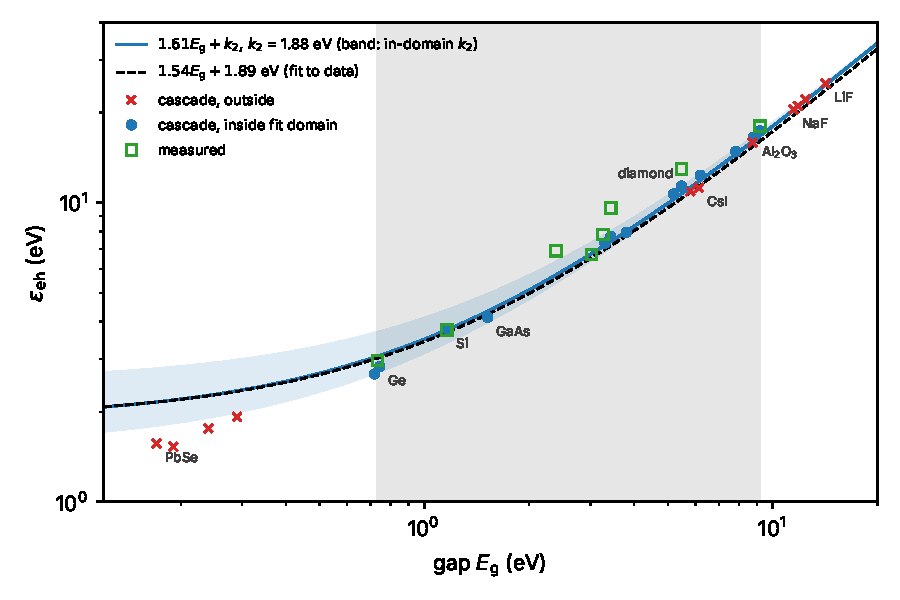
\includegraphics[width=\linewidth]{figures/ch18/limit18_4c.pdf}
\captionof{figure}{Pair energy against the gap. Solid line: \cref{eq:18.4-linear} with the silicon value $k_2 = \SI{1.88}{eV}$; band: $k_2$ over the crystals inside the fit region, 1.51 to \SI{2.53}{eV}. Dashed: the empirical line. Circles: the cascade with the constant \cref{eq:18.4-AAB} for the 24 crystals of Griffin and coworkers~\cite[Table~I]{griffin2020multichannel} (gap and highest optical phonon energy; silicon, germanium and GaAs at their low-temperature gaps of \cref{tab:3-materials}); filled inside the fit region $0.003 \le \lambda_{\mathrm{AB}} \le 100$, $0.01 \le w_{\mathrm{AB}} \le 0.1$ of \cref{eq:18.4-fit}, crosses outside it. Squares: measured pair energies of \cref{tab:18-valid} and silicon. Gray: the gaps of the measured crystals, 0.73 to \SI{9.2}{eV}. Slopes fitted for seed energies of 12.5 to $25\Eg$ (30 to $60\Eg$ for $\lambda_{\mathrm{AB}} > 5$), a window that changes the silicon value by less than \SI{0.03}{\percent} against the 20 to $40\Eg$ of \cref{tab:18-pairs}.}\label{fig:18-limit-c}
\par}
\smallskip
Outside the fit region, the law with each crystal's own $k_2$ still follows the cascade to \SI{1.4}{\percent} for these 24 crystals, but there it extrapolates the model beyond any comparison with data: the lead salts and InSb have $\lambda_{\mathrm{AB}} > 200$, and the halides and fluorides a phonon step below $0.006\Eg$.
\end{limitbox}

The linear law of the cascade and the empirical line have the same form for different reasons. The empirical constant 1.89 lies inside the range of $k_2$ and close to the value for silicon. The empirical slope 1.54 is below the model's 1.61, pulled down by diamond and the nitrides, for which the model with the silicon constant gives too little (\cref{sec:18.4-range}). Nielsen and Fischetti note that the measured $\varepsilon_{\mathrm{eh}}(\Eg)$ is not linear~\cite[Sect.~II]{nielsen2026first}; in the model, the nonlinearity comes from $k_2$, which changes from crystal to crystal with the phonon energy.

\begin{workedexample}{Pair energy of GaAs from the linear law}\label{we:18-gaas}
A GaAs detector at millikelvin has $\Eg = \SI{1.52}{eV}$ (\cref{tab:3-materials}) and a longitudinal optical phonon at $\omega_{\mathrm{AB}} = \SI{36.35}{meV}$ (\cref{sec:5.5}). With \cref{eq:18.4-AAB},
\begin{equation*}
  \lambda_{\mathrm{AB}} = \frac{5.703}{1.52^3} = 1.624, \qquad w_{\mathrm{AB}} = \frac{0.03635}{1.52} = 0.02391 .
\end{equation*}
The combination in \cref{eq:18.4-fit} is $\lambda_{\mathrm{AB}}w_{\mathrm{AB}}^{0.9637} = 0.04448$, and its power $0.2403$ is 0.4733. Then
\begin{equation*}
  \frac{\varepsilon_{\mathrm{eh}}}{\Eg} = 1.612 + 2.329\times0.4733 = 2.714, \qquad
  \varepsilon_{\mathrm{eh}} = 2.714\times\SI{1.52}{eV} = \SI{4.125}{eV} .
\end{equation*}
In the form \cref{eq:18.4-linear}, $1.61\Eg = \SI{2.45}{eV}$ and $k_2 = \SI{1.68}{eV}$, smaller than silicon's \SI{1.88}{eV} because the GaAs phonon carries 0.58 of the silicon phonon energy. The cascade itself yields \SI{4.132}{eV} (\cref{tab:18-pairs}), so the fit costs \SI{0.2}{\percent}. The empirical line gives \SI{4.23}{eV}. At the room-temperature gap of \SI{1.42}{eV} the linear law gives \SI{3.96}{eV}, against the measured value of about \SI{4.2}{eV}~\cite[Fig.~1]{nielsen2026first}; the difference is the residual of the model in \cref{tab:18-pairs}, carried through the fit. For a GaAs detector the defensible pair energy is therefore $\approx\SI{4.1}{eV}$ with an uncertainty set by the model's residuals, not by the fit.
\end{workedexample}

\subsection{The validated range}\label{sec:18.4-range}

\Cref{tab:18-valid} compares the cascade with the measured pair energies of seven crystals besides silicon, which fixes the constant. The inputs are the gap and the highest optical phonon energy of each crystal, longitudinal for the SiC polytypes.

\begin{table}[tbp]
\caption{Pair energies of the cascade with the silicon constant \cref{eq:18.4-AAB} against measurements. Inputs: germanium as in \cref{tab:18-pairs} (\SI{77}{K}); diamond, GaN and $\alpha$-quartz, gap and highest optical phonon energy of Griffin and coworkers~\cite[Table~I]{griffin2020multichannel}; the SiC polytypes, gap and longitudinal optical energy of Griffin and coworkers~\cite[Table~I]{griffin2021sic}. Measurements: germanium~\cite[Sect.~4.3]{mei2020impact}; diamond, the inverse-variance mean of four measurements (13.1, 13.25, 13.05 and \SI{12.82}{eV}) compiled by Nielsen and Fischetti~\cite[Sect.~III]{nielsen2023thermalization}; 4H-SiC~\cite{gsponer2023measurement}; 6H-SiC as quoted by Griffin and coworkers~\cite[Table~I]{griffin2021sic}; 3C-SiC and SiO$_2$ as quoted by Nielsen and Fischetti~\cite[Table~II]{nielsen2026first}; GaN, electron-beam induced current, as quoted by Nielsen and coworkers~\cite[Sect.~IV]{nielsen2023first}. Residual: model over measured, minus one. Last column: the density-functional full-band Monte Carlo of Nielsen and coworkers~\cite[Table~II]{nielsen2026first}, \cite[Sect.~III]{nielsen2023thermalization}, \cite[Sect.~IV]{nielsen2023first}.}
\label{tab:18-valid}
\centering\footnotesize\setlength{\tabcolsep}{3pt}
\begin{tabular}{lcccccccc}
\toprule
 & $\Eg$ (eV) & $\omega_{\mathrm{AB}}$ (meV) & $\lambda_{\mathrm{AB}}$ & $w_{\mathrm{AB}}$ & model (eV) & measured (eV) & residual & full band (eV) \\
\midrule
Ge & 0.735 & 37.6 & 14.4 & 0.051 & 2.815 & 2.96 & $-\SI{4.9}{\percent}$ & -- \\
3C-SiC & 2.39 & 120.5 & 0.42 & 0.050 & 6.121 & 6.90 & $-\SI{11.3}{\percent}$ & 6.6 \\
6H-SiC & 3.02 & 120.0 & 0.21 & 0.040 & 7.167 & 6.7 & $+\SI{7.0}{\percent}$ & -- \\
4H-SiC & 3.26 & 120.0 & 0.16 & 0.037 & 7.565 & $7.83 \pm 0.02$ & $-\SI{3.4}{\percent}$ & 7.3 \\
GaN & 3.43 & 88.9 & 0.14 & 0.026 & 7.694 & 9.59 & $-\SI{19.8}{\percent}$ & 8.9 \\
diamond & 5.47 & 161 & 0.035 & 0.029 & 11.357 & 12.95 & $-\SI{12.3}{\percent}$ & 12.87 \\
SiO$_2$ & 9.2 & 149 & 0.0073 & 0.016 & 17.373 & 18.0 & $-\SI{3.5}{\percent}$ & 16.7 \\
\bottomrule
\end{tabular}
\end{table}

Over the seven crystals the residuals run from $-\SI{19.8}{\percent}$ to $+\SI{7.0}{\percent}$, with a mean of $-\SI{6.9}{\percent}$ and a root mean square of \SI{10.5}{\percent}. The model is good to \SI{7}{\percent} for germanium, 4H- and 6H-SiC and quartz, and it falls short by 11 to \SI{20}{\percent} for 3C-SiC, diamond and GaN. Six of the seven residuals are negative, as are the residuals of germanium and GaAs in \cref{tab:18-pairs}: with the silicon constant the model tends to give too little heat per pair. The likeliest cause of the negative residuals is the universal constant, since the light-atom and polar lattices that the model misses most have phonon couplings unlike the couplings of silicon, but the comparison does not prove that the constant is the cause. The density-functional full-band Monte Carlo does better for diamond, 3C-SiC and GaN and worse for 4H-SiC and quartz, and it has no fitted constant. Its \SI{3.1}{eV} for silicon (\cref{sec:18.4-model}), \SI{17}{\percent} below the \SI{3.749}{eV} at \SI{123}{K}, shows that it is not yet a calibration-free substitute either.

The Fano factor is barely tested beyond silicon. The germanium measurements span a factor two, and the only wide-gap values, both for 4H-SiC, disagree with each other: $F_{\mathrm{eh}} = 0.1$ from a linewidth and an upper limit of 0.04 from another, as compiled by Gsponer and coworkers~\cite[Table~2]{gsponer2023measurement}. The model gives 0.093 for 4H-SiC. If the upper limit holds, the model fails for 4H-SiC, since 0.04 lies below every Fano factor the cascade produces in this section; a linewidth limit, however, rests on subtracting the noise from the measured width~\cite[Eq.~(3)]{gsponer2023measurement}, and an overestimated noise drives the limit down. Which of the two 4H-SiC values applies cannot be decided from the published data.

These comparisons define the \emph{validated range} of the cascade model: the region of phonon strength and phonon step spanned by the crystals with a measured pair energy, $0.007 \le \lambda_{\mathrm{AB}} \le 14.4$ and $0.016 \le w_{\mathrm{AB}} \le 0.054$, gaps from 0.73 to \SI{9.2}{eV}. Inside the validated range a model pair energy carries the spread of the residuals, $-20$ to $+\SI{7}{\percent}$, with the lower part more likely for light-atom and polar crystals. Of the crystals ranked in \cref{chap:17}, silicon, germanium, GaAs, diamond, quartz, CaWO$_4$, AlN, GaN and ZnO lie inside the range (\cref{fig:18-limit-c}). Sapphire and MgO lie just outside, with phonon steps of 0.012 and 0.011, and GaSb at its edge, with $\lambda_{\mathrm{AB}} = 15.3$.

Three groups lie well outside the validated range. The alkali halides and the fluorides, NaI, CsI, NaCl, LiF, NaF, CaF$_2$ and MgF$_2$, have phonon steps of 0.0016 to 0.006 of the gap. A carrier near threshold then emits hundreds of phonons before it ionizes, and no measured crystal samples a regime with so many phonons per ionization. The halides and fluorides have narrow anion valence bands, which confine the holes far more than in any validated crystal and which the model treats without a cutoff. They also bind excitons by an eV or more. A carrier between $\Eg - E_x^b$ and the impact-ionization threshold can create a bound pair directly; the cascade of \cref{sec:18.1} has no channel for this direct exciton creation, and whether a bound exciton counts as a pair depends on the readout (\cref{sec:18.5}). The lead salts and InSb have gaps below \SI{0.3}{eV} and $\lambda_{\mathrm{AB}}$ from 230 to 1160: their cascades are dominated by phonons, and at gaps this small, two processes absent from the model, Auger recombination and scattering by free carriers, can compete with impact ionization. For the crystals of these three groups the model pair energies in \cref{fig:18-limit-c} are estimates without a measured anchor, for example \SI{25.0}{eV} for LiF, \SI{20.5}{eV} for NaF, \SI{11.2}{eV} for CsI and \SI{1.56}{eV} for PbSe. Any guide to new targets must mark these pair energies as estimates. Neither the pair energy nor the Fano factor of sapphire, CaWO$_4$, LiF or NaF has been measured.
